
In letteratura ci si riferisce al termine ``processo'' come ad una istanza di un programma eseguito in modo sequenziale (che può essere o meno multithread in base al sistema operativo) su un processore. Tale concetto non è da confondersi con il concetto di thread, anche se in alcuni casi può coincidere con il processo.

In generale, si considerano i vari processi come entità concorrenti all'uso delle risorse del sistema (CPU, ram, I/O, etc..). Il sistema operativo gestisce l'accesso alle risorse, ed offre gli strumenti per controllare i processi, attraverso l'uso di ``segnali''. 

Tutti i processi vengono identificati all'interno del sistema attraverso un PID (Process IDentifier o identificativo di processo), ovvero un numero progressivo che solitamente va da 1 a 32768 (\directory{/proc/sys/kernel/pid\_max}). 

Il numero PID assunto da un processo non è predicibile, ma è noto che i primi PID sono relativi a processi di sistema, mentre il processo con PID 1 è sempre il processo di \textbf{init}.

All'infuori di \textbf{init}, tutti i processi presenti nel sistema, sono in un rapporto parentale con altri; ogni processo, nel momento in ``lancia'' (fork) un altro processo, diventerà il processo ``padre'' del processo lanciato. Contestualmente, il processo lanciato diventerà il processo ``figlio'' del processo chiamante.

La struttura padre/figlio dei processi offre una ottima struttura gerarchica di controllo dei processi. 

Alcune definizioni

\begin{itemize}
 \item Processo padre: processo che esegue una chiamata di tipo \textit{``fork()''} (seguita spesso da una \textit{exec()})
 \item Processo figlio: processo creato dalle chiamate del processo figlio
 \item Processo orfano: Processo che ha perso il processo padre, e viene ``adottato'' da init (re-parenting)
 \item Processo zombie (defunct): processo figlio sul quale il processo padre non ha eseguito la chiamata di wait() per leggerne il valore di ritorno. Per questo motivo il PID risulta ancora nella lista processi.  
\end{itemize}

Il sistema di comunicazione tra i processi ed il sistema è basato su notifiche asincrone definite segnali. A seguire alcuni di quelli definiti dallo standard POSIX (Portable Operating System Interface for Unix):

\begin{itemize}
 \item SIGHUP (1): Chiusura di un terminale.
 \item SIGINT (2): Interruzione da tastiera
 \item SIGQUIT (3): Segnale di uscita dalla tastiera
 \item SIGILL (4): Istruzione illegale (Illegal instruction)
 \item SIGABRT (6): Segnale di abbandono (abort)
 \item SIGFPE (8): Eccezione in virgola mobile
 \item SIGKILL (9): Termina il processo
 \item SIGSEGV (11): Riferimento in memoria non valido (segmentation fault)
 \item SIGPIPE (13): Broken Pipe
 \item SIGTERM (15): Segnale di terminazione
 \item SIGCHLD (20,17,18): Processo figlio terminato.
 \item SIGSTOP (17,19,23): Segnale di stop del processo
 \item SIGTSTP (18,20,24): Segnale di stop da tastiera
\end{itemize}


Il \textbf{SIGKILL} ed il \textbf{SIGTERM}, se pur simili, operano in modo diverso: il segnale di KILL, corrisponde ad una chiusura immediata, e non può essere ignorato. Il segnale di TERM invece consente al processo di eseguire le operazioni di uscita.  

Tutti i segnali possono essere intercettati, bloccati o ignorati, ad eccesione del segnale SIGKILL(9) e SIGSTOP(

Il comando per inviare i segnali ai vari processi è noto come \textit{kill}, e prende il nome dal segnale n. 9, erroneamente considerato il segnale di default del comando, che invece è il SIGTERM(15).

\begin{verbatim}
 $ kill -9 2345
 $ kill 2346 2349
\end{verbatim}

\subsection{Priorità}

Lo scheduler è quella parte dei sistema operativo che garantisce la concorezza alle varie risorse hardware. Per motivi di effecienza computazionale gli scheduler hanno un comportamento non predicibile, tuttavia è possibile influenzare il suo comportamento sfruttando il meccanismo della priorità.

La priorità consente di stabilire un ordine di esecuzione preferenziale, tale da garantire ai singoli processi un diverso accesso alle risorse (in particolare il processore). Nei sistemi di derivazione Unix, vale il concetto di \textbf{``niceness''}; si tratta di un valore inversamente proporzionale alla priorità. Minore è il valore di niceness, maggiore è la priorità, e viceversa. 
Alcuni valori di niceness (da -20 a -1) sono ad uso esclusivo dell'utente amministratore (root), questo per motivi di sicurezza ed efficienza del sistema operativo.  A meno di poche eccezioni, i processi partano con un valore di niceness uguale per tutti considerato come default (solitamente 0).

\begin{figure}[!ht]
 \centering
 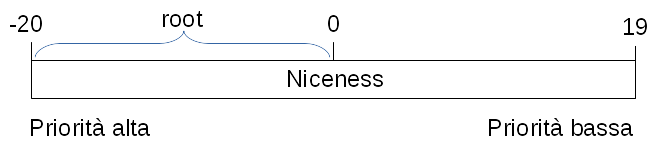
\includegraphics[scale=0.65]{Immagini/niceness.png}
 \label{fig:Niceness}
 \caption{Priorità}
\end{figure}

Due comandi tipici per impostare e reimpostare la priorità ad un processo sono rispettivamente il comando \textbf{nice} e \textbf{renice}. Ad esempio

\begin{verbatim}
 $ nice -10 /usr/bin/firefox
 $ renice -5 2345
\end{verbatim}


\subsection{System Monitor}

\begin{figure}[!ht]
 \centering
 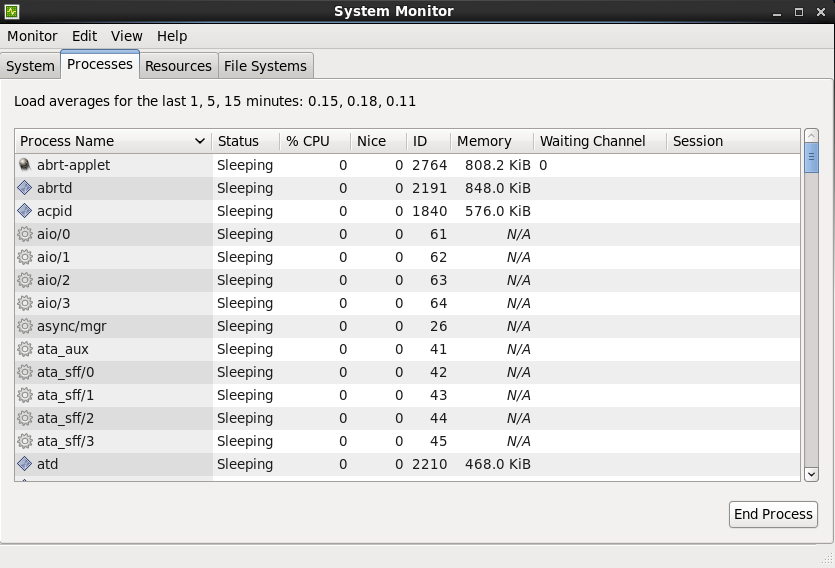
\includegraphics[scale=0.4]{Immagini/sys_mon1.png}
 \label{fig:System Monitor}
 \caption{System Monitor}
\end{figure}

System Monitor (gnome-system-monitor), presente nel menu alla voce \menu{Applications > System Tools > System Monitor}, è una pratica applicazione da UI, che consente di svolgere numerose operazioni

\begin{itemize}
 \item Visualizzare tutti i processi
 \item Visualizzare l'uso delle risorse (RAM, CPU, dischi, rete)
 \item Cambiare priorità ai processi
 \item Inviare segnali ai processi (9 e 15)
 \item Controllare le risorse sfruttate da ogni singolo processo
 \item Visualizzare l'abero gerarchico dei processi
\end{itemize}


\subsection{Gestione processi da terminale}


\subsubsection{ps}

Il comando \textbf{ps} (process status) mostra i processi presenti nel sistema. Si tratta di un comando con un numero considerevole di opzioni. Per varie ragioni mantiene la compatibilità di opzioni sia con quelle definite POSIX, e quelle BSD. Per non confondere i due tipi di opzioni, sotto Linux si possono usare le opzioni di tipo BSD, omettendo il carattere ``-''. 

Alcune opzioni POSIX:

\begin{itemize}
 \item ``-e'': Tutti i processi di tutti gli utenti
 \item ``-f'': Tutte le informazioni relative ai processi
 \item ``-l'': Formato esteso delle informazioni
 \item ``-p [lista-pid]'': Visualizza le informazioni sui processi con i pid selezionati
\end{itemize}

Alcune opzioni BSD

\begin{itemize}
 \item ``a'': Tutti i processi di tutti gli utenti
 \item ``x'': Mostra processi che non hanno un terminale controllante
 \item ``u'': Formato con informazioni su uso CPU
 \item ``p [lista-pid]'': Visualizza le informazioni sui processi con i pid selezionati
\end{itemize}

Ad esempio, i due modi più utilizzati per visualizzare tutti i processi di sistema (con output leggermente differenti) sono

\begin{verbatim}
 $ ps aux
 $ ps -ef
\end{verbatim}

Il comando \textbf{pstree} mostra tutto l'albero ``geneaologico'' dei processi attivi nel sistema. 

\subsubsection{top}

Il comando \textbf{top} offre una valida alternativa utilizzabile da shell a System Monitor. Top infatti visualizza dinamicamente le informazioni sul sistema e sui processi attivi, ordinandoli per consumo di CPU (oppure di memoria), fornendo anche la possibilità di interagire con i processi.

\begin{itemize}
 \item ``h'': Guida del programma
 \item ``k'': Invio di un segnale ad un processo (kill)
 \item ``r'': Permette di cambiare la niceness di un processo (renice).
 \item ``1'': Mostra/Nasconde le informazioni divise per singolo core
 \item ``q'': Uscita dal programma
\end{itemize}

Ad oggi esistono varianti del comando top, che, pur non essendo di default, sono installabili in un secondo momento quali \textbf{atop} e \textbf{htop}.

